\documentclass[12pt]{report}
\usepackage[utf8]{inputenc}
\usepackage[russian]{babel}
%\usepackage[14pt]{extsizes}
\usepackage{listings}

% Для листинга кода:
\lstset{ %
language=python,                 % выбор языка для подсветки (здесь это С)
basicstyle=\small\sffamily, % размер и начертание шрифта для подсветки кода
numbers=left,               % где поставить нумерацию строк (слева\справа)
numberstyle=\tiny,           % размер шрифта для номеров строк
stepnumber=1,                   % размер шага между двумя номерами строк
numbersep=5pt,                % как далеко отстоят номера строк от подсвечиваемого кода
showspaces=false,            % показывать или нет пробелы специальными отступами
showstringspaces=false,      % показывать или нет пробелы в строках
showtabs=false,             % показывать или нет табуляцию в строках
frame=single,              % рисовать рамку вокруг кода
tabsize=2,                 % размер табуляции по умолчанию равен 2 пробелам
captionpos=t,              % позиция заголовка вверху [t] или внизу [b] 
breaklines=true,           % автоматически переносить строки (да\нет)
breakatwhitespace=false, % переносить строки только если есть пробел
escapeinside={\#*}{*)}   % если нужно добавить комментарии в коде
}

% Для измененных титулов глав:
\usepackage{titlesec, blindtext, color} % подключаем нужные пакеты
\definecolor{gray75}{gray}{0.75} % определяем цвет
\newcommand{\hsp}{\hspace{20pt}} % длина линии в 20pt
% titleformat определяет стиль
\titleformat{\chapter}[hang]{\Huge\bfseries}{\thechapter\hsp\textcolor{gray75}{|}\hsp}{0pt}{\Huge\bfseries}


% plot
\usepackage{pgfplots}
\usepackage{filecontents}
\usetikzlibrary{datavisualization}
\usetikzlibrary{datavisualization.formats.functions}

\begin{document}
 
%\def\chaptername{} % убирает "Глава"
\begin{titlepage}
	\centering
	{\scshape\LARGE МГТУ им. Баумана \par}
	\vspace{3cm}
	{\scshape\Large Лабораторная работа №6\par}
	\vspace{0.5cm}	
	{\scshape\Large По курсу: "Операционные системы"\par}
	\vspace{1.5cm}
	{\huge\bfseries «Реализация монитора Хоара «Читатели-писатели» под ОС Windows» (Hoare C.A.R.)\par}
	\vspace{2cm}
	\Large Работу выполнил: студент группы ИУ7-53Б Наместник Анастасия\par
	\vspace{0.5cm}
	\Large Преподаватель:  Рязанова Н. Ю.\par

	\vfill
	\large \textit {Москва, 2020} \par
\end{titlepage}

\newpage

На листингах 1,...,5 представлено многопоточное приложение, демонстрирующее реализацию монитора Хоара «Читатели-писатели».

\begin{lstlisting}[label=some-code,caption=Начальные установки]
#include <windows.h>
#include <stdbool.h>
#include <stdio.h>
#include <time.h>
#include <stdbool.h>

#define WHITE "\033[0m"
#define GREEN "\033[0;32m"

#define WRITERS 5
#define READERS 3
#define ITERATIONS_NUMBER 100
#define HANDLE_ERROR 1
#define THREAD_ERROR 2

HANDLE CanWrite;
HANDLE CanRead;
HANDLE MUTEX;
LONG SHARED_RESOURCE = 0;

bool active_writer = false;
LONG active_readers = 0;
LONG writers_queue = 0;  //quantity of writers waiting for CanWrite
LONG readers_queue = 0;  //quantity of readers waiting for CanRead

HANDLE writerThreads[WRITERS], readerThreads[READERS];
int writerID[WRITERS], readerID[READERS];
int value = 0;
\end{lstlisting}

\begin{lstlisting}[label=some-code,caption=Код подпрограммы main()]
int main(void)
{
    setbuf(stdout, NULL);
    srand(time(NULL));
    
    if (!(MUTEX = CreateMutex(NULL, FALSE, NULL)))
        return HANDLE_ERROR;
       
    if (!(CanWrite = CreateEvent(NULL, FALSE, FALSE, NULL)))
        return HANDLE_ERROR;
    if (!(CanRead = CreateEvent(NULL, FALSE, FALSE, NULL)))
        return HANDLE_ERROR;
    
    if (Create_Threads() == THREAD_ERROR)
        return THREAD_ERROR;
  
    WaitForMultipleObjects(WRITERS, writerThreads, TRUE, INFINITE);
    WaitForMultipleObjects(READERS, readerThreads, TRUE, INFINITE);
    
    for (int i = 0; i < WRITERS; i++)
        CloseHandle(writerThreads[i]);

    for (int i = 0; i < READERS; i++)
        CloseHandle(readerThreads[i]);

    CloseHandle(CanWrite);
    CloseHandle(CanRead);
    CloseHandle(MUTEX);
    
  return 0;
}
\end{lstlisting}

\begin{lstlisting}[label=some-code,caption=Код подпрограммы создания потоков]
int Create_Threads()
{
    DWORD id = 0; //thread id
    
    for (int i = 0; i < WRITERS; i++)
    {
        writerID[i] = i;
        if (!(writerThreads[i] = CreateThread(NULL, 0, &Write, writerID + i, 0, &id)))
            return THREAD_ERROR;
    }

    for (int i = 0; i < READERS; i++)
    {
        readerID[i] = i;
        if (!(readerThreads[i] = CreateThread(NULL, 0, &Read, readerID + i, 0, &id)))
            return THREAD_ERROR;
    }
    return 0;
}
\end{lstlisting}

\begin{lstlisting}[label=some-code,caption=Код подпрограмм создания и работы писателя]
void Start_Write()
{
    InterlockedIncrement(&writers_queue);
    
    if (active_readers > 0 || active_writer)
        WaitForSingleObject(CanWrite, INFINITE);
    
    InterlockedDecrement(&writers_queue);
    active_writer = true;
}

void Stop_Write()
{
  
    active_writer = false;
    
    if (WaitForSingleObject(CanRead, 0) != WAIT_OBJECT_0)
        SetEvent(CanRead);
    else
        SetEvent(CanWrite);
}

DWORD WINAPI Write(LPVOID Id)
{
    int id = *(int *)Id;
    
    for (int i = 0; i < ITERATIONS_NUMBER; i++)
    {
        int delay = rand() % 200;
        
        Start_Write();
        value++;
        printf("%sWriter with id = %d wrote %d. Delay = %d\n", GREEN, id, value, delay);
        Stop_Write();

        Sleep(delay);
    }
}
\end{lstlisting}

\begin{lstlisting}[label=some-code,caption=Код подпрограмм создания и работы читателя]
void Start_Read()
{
  
    InterlockedIncrement(&readers_queue);
  
    if (active_writer || WaitForSingleObject(CanWrite, 0) == WAIT_OBJECT_0)
        WaitForSingleObject(CanRead, INFINITE);
    
    WaitForSingleObject(MUTEX, INFINITE);
    
    InterlockedDecrement(&readers_queue);
    InterlockedIncrement(&active_readers);
    SetEvent(CanRead);
    
    ReleaseMutex(MUTEX);
}

void Stop_Read()
{
    InterlockedDecrement(&active_readers);
  
    if (active_readers == 0)
        SetEvent(CanWrite);
}

DWORD WINAPI Read(LPVOID Id)
{
    int id = *(int *)Id;
    
    for (int i = 0; i < ITERATIONS_NUMBER; i++)
    {
        int delay = rand() % 200;
        
        Start_Read();
        printf("%sReader with id = %d read %d. Delay = %d\n", WHITE, id, value, delay);
        Stop_Read();
        
        Sleep(delay);
    }
}
\end{lstlisting}

На рисунке 1 приведен результат работы программы.
\begin{center}
		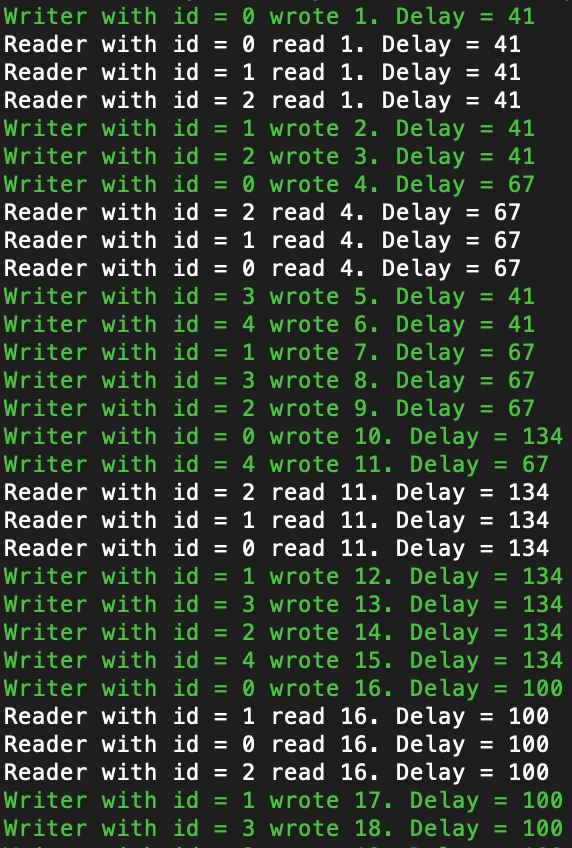
\includegraphics[scale=0.8]{pics/RW.png}
		
			Рис 1:  Результат работы программы 
\end{center}


\end{document}